\section{Desarrollo}

\subsection{Lexer}

Utilizamos los siguientes tokens con sus respectivas reglas
\begin{itemize}
	\item \textbf{DIVIDE}: El símbolo '/' para la división
	\item Los literales: \quotes{\sub \ \super \ () \{\}}
	\item \textbf{CHR}: Cualquier símbolo exceptuando los anteriores.
	\\Esto incluye:
	\begin{itemize}
		\item cualquier caracter a-z y A-Z
		\item +
		\item *
	\end{itemize}
\end{itemize}

\subsection{Gramática}

$ \mathcal{G} = \langle$ \{$E$, $UNARYEXP$, $SUPEREXP$, $SUBEXP$\},   \big \{$CHR$, $DIVIDE$, `_', `\super', `(', `)', `\{', `\}' \big \},   $\mathcal{P}$,   $E$ $\rangle $

\begin{figure}[h!] \centering
\begin{tabular}{lrrl}
$\mathcal{P}:$
& $E$  & \produces     & $UNARYEXP$ \\
& & \alsoproduces & $E \verb| | E$ \\
& & \alsoproduces & $E$ \textbf{DIVIDE} $E$ \\
& & \alsoproduces & $UNARYEXP \verb| ^ | UNARYEXP \verb| | SUBEXP$ \\
& & \alsoproduces & $UNARYEXP \verb| _ | UNARYEXP \verb| | SUPEREXP$ \\
& & \alsoproduces & $E \verb| DIVIDE | E$ \\
& $UNARYEXP$  & \produces     & \textbf{CHR} \\
& & \alsoproduces & ( $E$ ) \\
& & \alsoproduces & \{ $E$ \} \\
& $SUPEREXP$  & \produces     &  \verb| ^ | $UNARYEXP$ \\
& & \alsoproduces & $\lambda$ \\
& $SUBEXP$  & \produces     &  \verb| _ | $UNARYEXP$ \\
& & \alsoproduces & $\lambda$ \\


\end{tabular}
\caption{Producciones de la gramática}
\label{fig:gramatica}
\end{figure}

Siendo la gramática original la siguiente:

\begin{figure}
    \centering
    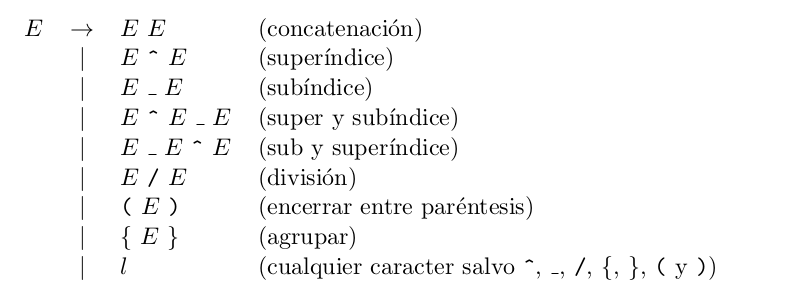
\includegraphics[width=0.9\textwidth, height=0.22\textheight, keepaspectratio]{gramoriginal}
    \caption{Gramática original a parsear según enunciado.}
    \label{fig:gram_original}
\end{figure}

Como \emph{PLY}, la herramienta que usamos tanto para el análisis lexicográfico (lexer) como para parsear, usa técnicas de tablas LALR, tuvimos que hacer algunas modificaciones sobre la gramática original para poder generar una tabla de dichas características. \newline

Una de ellas fue juntar las producciones \emph{"superíndice"} y \emph{"super y subíndice"} en una única usando un no-terminal nuevo $SUBEXP$ que pudiera ser anulable o generar el subíndice e idem para las producciones \emph{"subíndice"} y \emph{"sub y superíndice"}. De lo contrario una cadena con super y subíndices  como $A\super B\sub C$ podría ser generada produciendo primero un superíndice y luego un subíndice usando dos producciones tanto como usando una única producción. \newline

Otra manera de sortear este problema hubiera sido eliminando las producciones que combinan super y subíndices y usando ambas producciones de manera consecutiva, pero preferimos mantener las producciones ternarias sobre las binarias para facilitar el recorrido y "decorado" de la estructura sintáctica (sino no se nos complicaría distinguir estructuras de cadenas como $ A\sub \{B\super C\} $ ó $\{A\sub B\}\super C$ de las de $A\sub B\super C$). \newline

El otro cambio importante fue agregar otro no-terminal $UNARYEXP$ que genera producciones 'unarias' (paréntesis o llaves sobre una $E$, o un $CHR$). La idea viene de la necesidad de desambiguar expresiones como $E\super E\sub E$ que podrían ser generadas como $E \Rightarrow E \super  E\ SUBEXP \Rightarrow E\super E\sub E$ o como $E \Rightarrow  E \super  E\ SUBEXP \Rightarrow E \super  E \Rightarrow E\ \super  E\sub \ E\ SUPEREXP \Rightarrow E \super  E\sub \ E\ $. \newline

Como según el enunciado ni los '\super ' ni los '_' son asociativos y además $E\sub  E \super  E$ y $E\super  E \sub  E$ son equivalentes, viendo expresiones de la pinta $E_1 \sub  E_2 \super  E_3$ se puede ver que ninguno de los tres no-terminales pueden producir nunca otro subíndice o superíndice en el mismo 'scope' de paréntesis o llaves. Esto es porque siempre podríamos invertir el orden usando la equivalencia mencionada anteriormente de modo que se asocien dos de estos símbolos. \\
Tampoco pueden producir concatenaciones o divisiones porque '\super' y '_' tienen mayor precedencia que estos, por ejemplo la cadena $A\super BC$ (escribiendo los terminales $CHAR$ como sus valores para mayor claridad) no tiene la estructura de $A\super \{BC\}$ sino de $A\super B$ concatenado a $C$ \footnote{idem para subindexación} y en el caso de $A/B\super C\sub D$ primero se resuelve la indexación de B y luego la división por lo tanto la estructura se corresponde a $A/\{B\super C\sub D\}$ \footnote {idem si fuera concatenación}.

Con todos estos cambios aún seguimos teniendo problemas de tipo \emph{Shift/Reduce} y \emph{Reduce/Reduce} en nuestras tablas, que resolvimos declarando las siguientes precedencias:

Tabla de precedencia (en orden creciente)
\begin{itemize}
	\item \textbf{DIV} asociativa a izquierda

    \item '\{', '(' asociativas a izquierda
    \item \textbf{CHR} asociativa a izquierda
    \item CONCAT, asociativa a izquierda, pseudosímbolo para la concatenación
    \item \verb|'^'| no asociativa
    \item \verb|'_'| no asociativa
\end{itemize}

Las reglas de la concatenación, división e indexación siguen la descripción del enunciado mientras que las que se corresponden a $Primeros(E)$ sirven para resolver en favor de \emph{Shifts} cuando se llega al final de la expresión de una división y se está por ver una concatenación. (es decir, \textbf{DIV} tiene menos precedencia que los 'primeros' de $E$ y que las otras operaciones) y que se tome \emph{Reduce} cada vez que se vió una concatenación si se está por ver una expresión concatenada o de división \footnote{Esto en teoría alcanzaría con declarar a CONCAT como asociativa a izquierda y de mayor precedencia que la división, pero al parecer para que \emph{Yacc} pueda resolver conflictos comparando orden de precedencias de símbolos con órdenes de precedencias de producciones hace falta cierta completitud sobre las declaraciones de precedencia de los símbolos que puedan llegar a ser el token corriente al decidir si reducir o no usando una producción.}.

\subsection{AST}

\subsection{Atributos y SVG}
